\section{Mergesort}
O Mergesort é um algoritmo de ordenação estável baseado na técnica de divisão e conquista, proposto por John von Neumann em 1945. Essa técnica consiste em um processo recursivo de três etapas:
\begin{enumerate}
    \item Divisão: divide-se o problema em instâncias menores do mesmo problema.
    \item Conquista: resolve-se cada uma das instâncias definidas na etapa anterior.
    \item Combinação: combinam-se as soluções para resolver o problema original.
\end{enumerate}

Enquanto as etapas de divisão e conquista consistem apenas em algumas operações aritméticas e duas chamadas recursivas, a de combinação requer um pouco mais de atenção. Nesse momento, tem-se dois vetores ordenados, e é necessário juntá-los em apenas um vetor também ordenado, em um processo chamado intercalação, que aqui será referido pelo termo em inglês \textit{merge}.

\subsection*{Intercalação de vetores ordenados}
A implementação da operação \textit{merge} é mostrada em linguagem C abaixo. Ela assume que $v[l..m - 1]$ e $v[m..r - 1]$ estão ordenados. O resultado é que $v[l..r - 1]$ também ficará em ordem. A função CopiaVetor, na linha 2, copia os $r - l$ elementos de $v[l..r - 1]$ para o vetor auxiliar $v\_aux[l..r - 1]$. Doravante, essa função será usada de forma similar, sem mais explicações.

\lstinputlisting[language=C]{codigos/aux/merge.txt}

\subsection*{O algoritmo Mergesort}
Este trabalho traz uma implementação dividida em dois métodos. O primeiro é apenas uma interface que segue o mesmo padrão de assinatura dos métodos de ordenação mostrados anteriormente, e é responsável por alocar e liberar a memória auxiliar, além de invocar o segundo método. O segundo é uma implementação recursiva do algoritmo que executa as três etapas da técnica já mencionada. A função AlocaVetor usa malloc para alocar um vetor com o tamanho especificado e verifica se a alocação ocorreu com sucesso.

\lstinputlisting[language=C]{codigos/sup/2_mergesort.txt}

\begin{figure}[H]
\Caption{\label{fig:mergesort}Ilustração do Mergesort aplicado ao vetor $[19,2,17,3,13,5,11,7]$.}
\centering
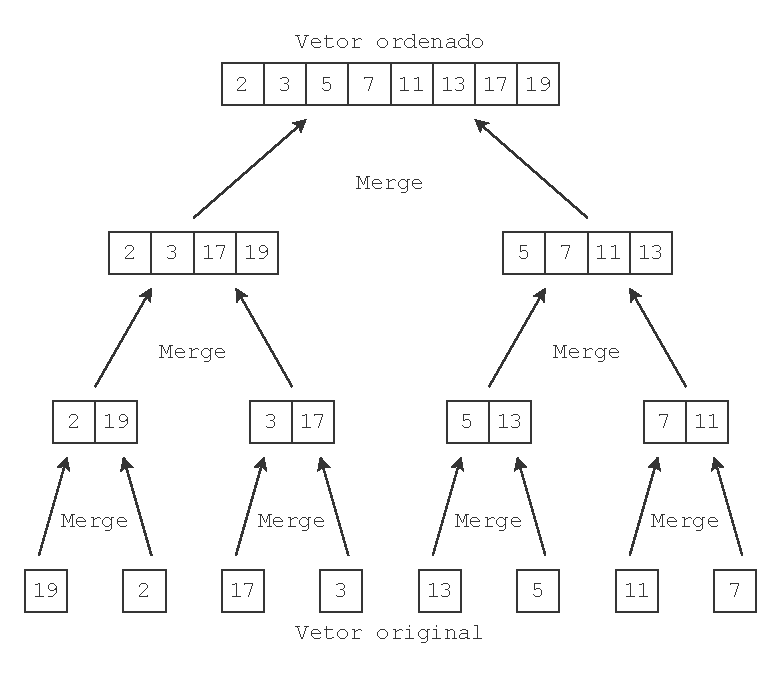
\includegraphics[scale=1.0]{figuras/pdf/mergesort.pdf}
\Fonte{Elaborado pelo autor}
\end{figure}

\subsection*{Corretude}
Observe que a base da recursão está bem definida, pois um vetor com menos de dois elementos já está ordenado. Note também que, em cada chamada, o vetor é dividido aproximadamente ao meio, e cada metade é ordenada recursivamente, sem deixar lacunas antes, entre ou depois de cada uma. Por fim, veja que a função Merge copia $v[l..r - 1]$ para $v\_aux[l..r - 1]$ e depois traz os elementos de volta para $v$, um por um, sempre escolhendo o menor que ainda não foi copiado. Como cada uma das etapas está correta, o Mergesort também está correto.

\subsection*{Desempenho}
Seja $T(n)$ o tempo necessário para ordenar um vetor de $n$ elementos utilizando o Mergesort. Temos então que:
\[
  T(n) = 
  \begin{cases}
      \Theta(1),              & n = 1    \\
      \underbrace{\Theta(1)}_{\text{Divisão}} + \underbrace{2T(n/2)}_{\text{Conquista}} + \underbrace{\Theta(n)}_{\text{Intercalação}}, & n > 1 
  \end{cases}
\]
Desta forma, podemos simplesmente dizer que para $n > 1$ e alguma constante $c$,
\[
  T(n) \;=\; 2T(n/2) + cn \;\;\;\Rightarrow\;\;\; T(n) \;=\; n\log_2 n + cn
\]
Portanto, o consumo de tempo do Mergesort é $\Theta(n\log_2 n)$. Já o de memória é $\Theta(n)$, devido ao vetor auxiliar utilizado.
